% used for market drawings
\newlength{\slotwidth}
\setlength{\slotwidth}{.103\textwidth}

\section{The Packet-by-Packet Market}
\label{sec:designs}

Our proposal for self-incentivizing networks is a speculative one. To
assess, preliminarily, whether such a scheme could work, we
conducted simulation experiments for a one-hop version of the system.

We describe here the design for a logically centralized
packet-by-packet market that allows anybody to contribute transmission
capacity between two nodes and be rewarded for it, as endpoints
purchase the right to send each packet from the market.

In these systems, the scarce resources of the communications links are
allocated not by TCP, AQM, or a traffic-engineering scheme. Instead,
the links are allocated by a tableau of simultaneous per-timeslice
auctions.

The principal contribution of our findings thus far is that a simple
market-based mechanism, where users bid for the opportunity to send
each packet, can recover schedules that closely approximate the
optimal shortest-remaining-time-first schedule across a contended link.

We discuss here the design for the simple market
(Section~\ref{ss:simplemarket}), our simulation and analytical
evaluation of this system (Section~\ref{ss:eval}), and finally our
unevaluated design for a ``multiresolution'' market that corrects
some of the problems in the simple design.

\subsection{Simple-Market Design}
\label{ss:simplemarket}

\begin{figure*}
\renewcommand{\arraystretch}{2}
\begin{tabular}[height=3in]{|*{8}{p{\slotwidth}|}}
\hline
Time: 0 & Time: 1 & Time: 2 & Time: 3 & Time: 4 & Time: 5 & Time: 6 & Time: 7 \\
\{(A, \$2.01)\} & \{(A, \$2.01)\} & \{(B, )\} & \{(B, )\} & \{(ISP, \$1)\} & \{(ISP, \$1)\} & \{(C, \$10)\} & \{(ISP, \$1)\} \\
\hline
\end{tabular}
\caption{An example snapshot of the ``simple market'' order book. User
A owns the first two time slots and has posted an offer to resel them
for \$2.01 apiece. User B owns the next two slots and has not posted
an offer to sell them. User C owns the slot at time 6 and has posted
an offer of \$10 to sell it. ``ISP'' owns the remaining slots with an offer of \$1 apiece.}
\label{f:simple_market}
\end{figure*}

Our goals for a market were as follows:
\begin{itemize}
\item Let anyone contribute capacity---the ability to transmit a
packet from point A to point B at a certain time.

\item Allow users to act selfishly to maximize their own utility
functions.

\item Allow users to buy, in advance, the right to send packets at a
particular time, which they can then resell. This could be used to
allow a user to construct a virtual link with a certain continuous
throughput.

\item Demonstrate that this system produces a good result globally.
\end{itemize}

Our ``simple'' market is composed of sequential, consecutive time
slots in which a packet can be delivered. Users are able to buy the
right to send a packet within a given time slot.  Once a user buys a slot,
they own a guarantee: if they deliver the packet to one
side of the link by the beginning of the slot, it will make it to the
next hop by the end of the slot interval. The slot owner can also post an offer to re-sell
the slot to another user for a given price.

Figure \ref{f:simple_market} gives an example of the state of the
market's order book---showing the sequential, simultaneous per-timeslice
auctions---at a given time.

The objectives of market users and their flows could vary greatly. In our simulations,
we have experimented with several types, outlined in Figure~\ref{f:user_types}.
\begin{figure*}
\begin{tabular}{|p{.25\textwidth}|p{.70\textwidth}|}
\hline
Flow Type & Objective \\
\hline
\hline
Flow-completion priority & Send $n$ packets, minimizing flow-completion time. \\
\hline
Isochronous flow & Send $n$ packets every $t$ milliseconds. \\
\hline
Deadline flow & Send $n$ packets by deadline $d$. \\
\hline
Evil user & Maximally reduce utility of another market user while
staying within a budget $c$. We discuss the problems of ``evil'' or
strategic bidders in Section~\ref{ss:evil}. \\
\hline
ISP & Simply posts offers to transmit packets; doesn't bid. \\
\hline
\end{tabular}
\caption{Flows and their Bidding-Control Protocols may come in a variety of flavors.}
\label{f:user_types}
\end{figure*}

\subsection{Implementation}
We implemented a range of bidding-control protocols, or BCPs, in
C++. These BCPs participate in the market, placing bids and offers to
maximize the objectives described in Figure~\ref{f:user_types} on
behalf of user flows.

We then built a market simulator, which takes a set of user BCPs
and executes them in round-robin order, giving them the current order
book and the list of packets actually transmitted on the link (so they
can see which opportunities they have ``won'').

At a given timestep, the simulator runs each BCP until all users have
stopped changing the order book, then advances time. When time
advances, any user owns the right to send a packet during front-most
slot in the order book is deemed to send a packet across the link. (If more than one
ISP has offered an opportunity at that slot, more than one packet
might be sent.) The simulation ends when all flows have
completed. We view this as a simplified, idealized model of what might
occur in a home router controlling, e.g., a contended cable-modem link.

\textbf{Flow-completion priority BCP:} The implementation of the
BCP for flows that care only about their completion time
(``flow-completion priority'' in Figure~\ref{f:user_types}) deserves
some further discussion. This type models a flow that arrives at a set
time and has a set number of packets $n$ to send. It tries to maximize
the utility function $U = -d - c$, where $d$ is the number of
timeslots until the \emph{last} packet is transmitted, and $c$ is the
total amount paid for slots.  Upon arrival, this user buys $n$
slots, choosing the best balance between cost and duration. Once slots have been
purchased, it posts an offer for each slot that it owns, offering
to sell the slot for \$.01
more than the negated loss of utility that the user would experience if it lost
that slot and had to buy the next-best one. We find that this mechanism
is generally sufficient to closely approximate the shortest-remaining-time-first schedule.

\subsection{Simple-Market Evaluation}
\label{ss:eval}

\begin{figure}
%\vspace{\baselineskip}
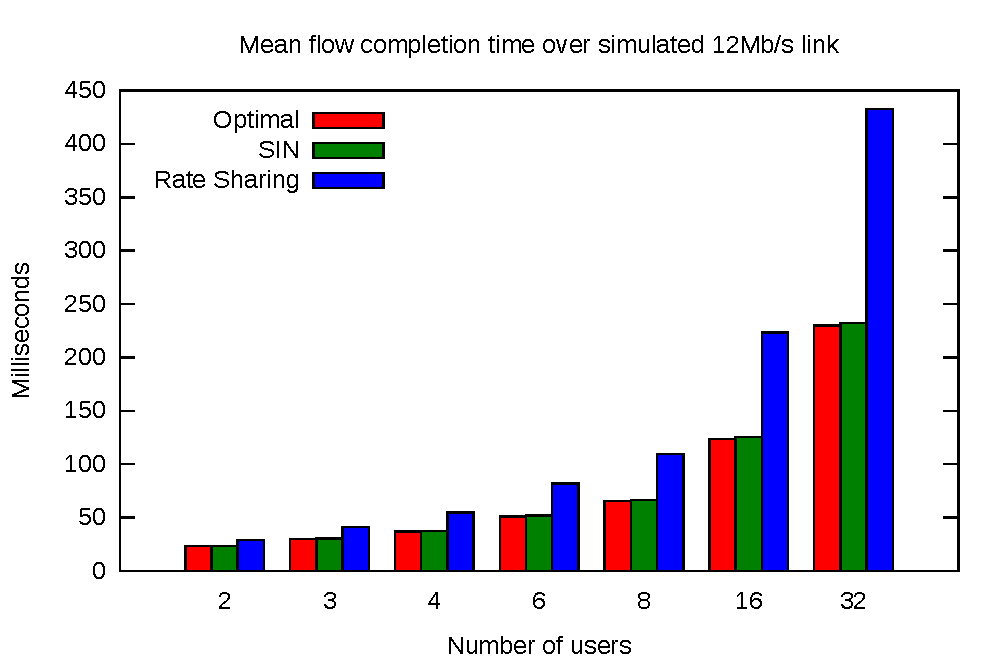
\includegraphics[width=\columnwidth]{plots/delay_over_srtf.pdf}
\caption{In simulations where every user runs the flow-completion priority BCP,
the simple self-incentivizing network (SIN) closely approximates the
optimal shortest-remaining-time-first (SRTF) schedule and outperforms
a policy of perfect rate sharing among live flows, such as achieved by
an idealized TCP.}
\label{f:delay_over_srtf}
\end{figure}

\begin{figure}
%\vspace{\baselineskip}
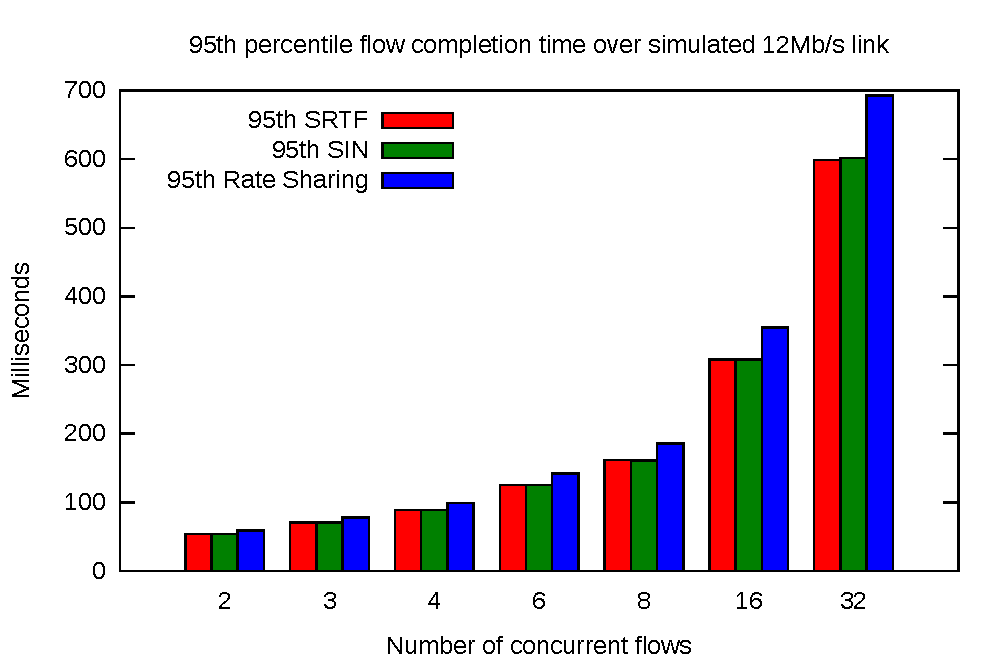
\includegraphics[width=\columnwidth]{plots/95th_delay_over_srtf.pdf}
\caption{The self-incentivizing network also performs well in terms of tail FCT.}
\label{f:95th_delay_over_srtf}
\end{figure}

We simulated the results of running the simple market with
flow-completion priority users that would arrive at time $t$, drawn
from a uniform distribution on $[0, 39]$, with a flow length drawn
from a uniform distribution on $[0, 40]$ packets.
Figures~\ref{f:delay_over_srtf} and \ref{f:95th_delay_over_srtf} show
the result of running the simulation with between 2~and~32 concurrent
flows. A single ISP offers to send one packet per millisecond,
resulting in a capacity of 12~Mb/s, and posts these offers initially at \$1 per
packet.

We compare the mean flow duration achieved among greedy users by our
market mechanism against the shortest-remaining-time-first schedule
(SRTF). We also compared against an equal rate-sharing or round-robin
schedule, such as would be achieved by an idealized TCP.

It is well known that SRTF achieves
the minimum mean flow duration for an online algorithm with
known job durations~\cite{karger10,bansal01}.

As our figures show, the greedy BCPs in our simulation converge on a
near-optimal mean-flow-duration schedule for the link. For all numberss
of users, the SIN schedule had a mean flow duration that was less
than 1\% higher than SRTF.

\subsubsection{The Exposure Problem}

Unfortunately, in simulation it is possible that a user BCP would have
had a higher utility at the end if it had refused to put offers on slots it had purchased.

This is possible because our flow-completion priority BCP bases its
offer prices on the offer prices of the slots that it would buy instead
if their slot were sold, but they are not always able to purchase
those replacement slots for those prices (for example if they were
sold to someone else who raised the price in the meantime). In an attempt to avoid
this, users frequently re-price their slots, but unless their price
can instantly reflect a price change, this possibility of a user
hurting their final utility is unavoidable with our current market.

This is a serious problem with the simple market: why would a greedy
user, who has just purchased a slot, offer to resell that slot if it
were likely that this would \emph{decrease} its ultimate utility?
Fear of this outcome could lead users to post inflated offer prices, or no offers at all, on
slots they own, which would reduce the quality of schedules the market
produces. In auction theory, similar issues are known as 
\emph{exposure problems}~\cite{milgrom00,
englmaier06}, where slot prices are dependent on one other.

\subsubsection{The problem of evil}
\label{ss:evil}
We sought to exploit this problem as much as possible, and found that
disappointment can be arbitrarily bad in the case of an ``evil user'':
one whose sole objective is to reduce the utility of another
user.

An evil user could maximally reduce the utility of a flow-completion
time BCP for the cheapest cost, by buying the next $m$ slots after the
last packet of the flow-completion priority BCP without putting up
offers for any slots, and then buying the cheapest packet that the
flow-completion priority BCP has offered for sale before it has a
chance to re-price that offer.

To finish its flow, the flow-completion priority BCP
will then have to buy another packet much later, which reduces its
utility by at least $m$.

The amount of money spent by the evil user is typically only a
constant offset from the amount of pain it is able to inflict on
another user by exploiting the Exposure Problem---a serious
weakness. A better market would eliminate the Exposure Problem or make
disruption more costly.

\subsubsection{Communication overhead}

\begin{figure}
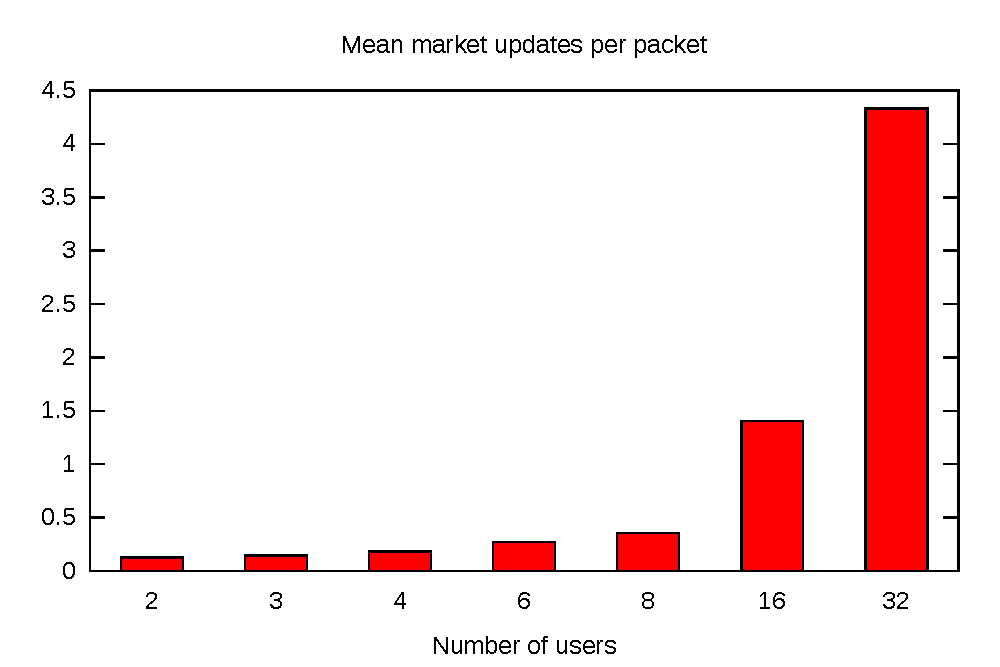
\includegraphics[width=\columnwidth]{plots/num_market_updates.pdf}
\caption{Mean number of sets of slot purchases made by flow-completion
priority BCPs in simulation.}
\label{f:num_market_updates}
\end{figure}

Another problem with the simple market is that it can take many rounds
of bidding
to converge on a quiescent order book, where no user wants to buy more slots. In
simulation, flow-completion priority BCPs would buy back and forth from each other many times, making small price adjustments throughout.  
Figure~\ref{f:num_market_updates} shows the number times a user bought a set of packets on the market, or market updates, per packet sent in the simulations from in Figure~\ref{f:delay_over_srtf}.
More contention between slots increased the number of market updates
required.

We can envision scenarios where this number of roundtrips might be
acceptable---for example, if the market is run very close to the users
(e.g.~at a home cable modem) and the link that is being adjudicated is
much slower than the link used to access the logically-centralized
market. But clearly it would be preferable to reduce the number of
roundtrips to the order book.

%TODO improve below sentence
\subsection{Multiresolution market design}
\label{ss:multires}
The weaknesses we encountered with the simple market have led us to our current design:


\begin{comment}
TODO

\begin{figure*}
\renewcommand{\arraystretch}{2}
\begin{tabular}[height=3in]{|*{8}{p{\slotwidth}|}}
\hline
\multicolumn{8}{|c|}{}\\
\hline
\multicolumn{4}{|c|}{} &\multicolumn{4}{c|}{} \\
\hline
\multicolumn{2}{|c|}{} &\multicolumn{2}{c|}{} &\multicolumn{2}{c|}{} &\multicolumn{2}{c|}{}\\
\hline
Time: 0 & Time: 1 & Time: 2 & Time: 3 & Time: 4 & Time: 5 & Time: 6 & Time: 7 \\
\{(A, \$2.01)\} & \{(A, \$2.01)\} & \{(B, )\} & \{(B, )\} & \{(ISP, \$1)\} & \{(ISP, \$1)\} & \{(C, \$10)\} & \{(ISP, \$1)\} \\
\hline
\end{tabular}
\caption{Multiresolution market order book.}
\label{f:multiresolution _market}
\end{figure*}

\end{comment}
